\section{Experiments}
\subsection{Stress-buffering Effect of Positive Events}
\label{subsec:experiment}
\begin{table}[h]
\begin{center}
\caption{\small{Quantify the stress-buffering effect of scheduled positive events applying KTS model (the KNN-based two sample method adopted in this research) and baseline method.}}
\label{tab:schedule}
\resizebox{0.45\textwidth}{13mm}{
\small{
\begin{tabular}{lccccc}
\toprule
&	practical	&	         	&	new year	&	sports	&	\\
&	activity	&	holiday	&	party	&	meeting	&	all	\\
\midrule
size of U-SI	&	219 	&	339 	&	235 	&	226 	&	1,019 	\\
Pearson         &55.65\%	&	70.97\%	&	56.45\%	&	54.84\%	&	65.32\% \\
KTS             &54.52\%	&	78.39\%	&	63.39\%	&	58.74\%	&	69.52\% \\
\bottomrule
\end{tabular}
}
}
\end{center}
\end{table}
Basically, we explored the stress-buffering effect of specific positive events based on the framework in section \ref{sec:frame}.
Four scheduled positive events were adopted:
practical activity, holiday, new year party and sports meeting.
Table \ref{tab:schedule} showed the experimental results,
where 54.52\%, 78.39\%, 63.39\%, 58.74\% significant stress-buffering effect were detected for
each of the four scheduled positive events, with the total ratio to 69.52\% ($\alpha$ =1.96 for p=0.025).
Here Pearson correlation algorithm was applied to compare with the statistical model in section \ref{sec:frame2}.
The Euclidean metric was used to calculate the distance between two $n$ dimension points $X$ and $Y$.
Experimental results showed that our KNN-based two sample method (denoted as KTS) outperformed the baseline method
with the best improvement in event \emph{new year party} to 10.94\%, and total improvement to 6.00\%.

\begin{figure}[h]
\centering
\includegraphics[width=\linewidth]{figs/cor.eps}%figs/correlation2.eps
\caption{\small{ Subgraph (a) showed statistical value $\alpha$ of each group of measures.
Subgraph (b) showed stress-buffering effect on five dimensions of stress.}}
\label{fig:correlation}
\end{figure}

Stress-buffering effects measured by three groups of microblog characteristics and towards five dimensions of stressor events were shown in box-plots \ref{fig:correlation},
using the statistical value $\alpha$ computed through KTS method.
Results showed the stress-buffering pattern of positive events
was significantly correlated with posting behaviors (ratio = 83.06\%, n=103, SD=1.96),
stress change modes (ratio = 74.19\%, n=92, SD=2.04) and linguistic expressions (ratio = 77.42\%, n=96, SD=2.07).
Positive events conducted most significant stress-buffering impact on 'family life' (ratio = 84.68\%, n=105, SD=2.72),
followed by 'peer relationships' (ratio = 79.03\%, n=98, SD=4.04) and 'academic' (ratio = 68.55\%, n=85, SD=2.71) dimensions.
Statistics $\alpha$ in 'peer relation'
exhibited the highest 75th percentile while the lowest 25th percentile,
showing a relatively random and unstable stress-buffering effect on this dimension.
Comparing the hypothesis test results on scheduled positive events (ratio = 69.52\%)
and automatically extracted positive events (ratio = 74.21\%),
the result indicated the feasibility of automatically extracting positive events from microblogs.

Next,
to verify monotonous changes of stress intensity when an positive event impacted a stressful interval,
for each interval in SI and U-SI sets,
we quantified its monotonous stress changes by comparing with the front and rear adjacent intervals, respectively.
Four situations proposed in section \ref{sec:mono} were considered and compared in table \ref{tab:fontrear}.
The ratio of intervals detected with monotonous increase from the front interval to current stressful interval $I$ (denoted as \emph{front$ \rightarrow$ I}),
and ratio of monotonous decrease from $I$ to its rear interval (denoted as \emph{I $\rightarrow$ rear}) were summarized.
Under the effect of positive events,
the ratio of intensive stress increase in \emph{front$ \rightarrow$ I} was decreased from 78.51\% to 70.17\%;
and the ratio of intensive stress decrease in \emph{I $\rightarrow$ rear} was decreased from 79.55\% to 75.13\%.
The most obvious monotonous decrease in \emph{front$ \rightarrow$ I} was conducted by positive events in family life dimension (12.89\% reduction);
and the most obvious monotonous decrease in \emph{front$ \rightarrow$ I} was also conducted by positive events in family life dimension (6.65\% reduction).
The experimental results indicated the effectiveness of the two sample method for quantifying the effect of positive events,
and the rationality of the assumption that positive events could help ease stress of overwhelmed adolescents.


\begin{table*}
\caption{Compare stress prediction performance under three groups of stress-buffering measures.}
\begin{minipage}{\linewidth}
\centering
\resizebox{\textwidth}{20mm}{
\begin{tabular}{l cccc cccc cccc cccc} \\\hline%\toprule
\multirow{2}{1cm}{}&\multicolumn{4}{c}{None}
    &\multicolumn{4}{c }{Positive (L)}
    &\multicolumn{4}{c }{Positive (S)}
    &\multicolumn{4}{c}{Positive (P)}\\
    &\scriptsize{MSE} &\scriptsize{RMSE} &\scriptsize{MAPE} &\scriptsize{MAD}
    &\scriptsize{MSE} &\scriptsize{RMSE} &\scriptsize{MAPE} &\scriptsize{MAD}
    &\scriptsize{MSE} &\scriptsize{RMSE} &\scriptsize{MAPE} &\scriptsize{MAD}
    &\scriptsize{MSE} &\scriptsize{RMSE} &\scriptsize{MAPE} &\scriptsize{MAD} \\\midrule					
School life
&   0.0856 	&	0.2926 	&	0.4852 	&	0.1146	&	0.0259 	&	0.1609 	&	0.2991 	&	0.0923 	
&	0.0297 	&	0.1723 	&	0.3135 	&	0.0899 	&	0.0223 	&	0.1493 	&	0.3438 	&	0.0931 	\\
Romantic
&   0.0703 	&	0.2651 	&	0.3555 	&	0.1083 	&	0.0291 	&	0.1706 	&	0.2832 	&	0.0919 	
&	0.0379 	&	0.1947 	&	0.2941 	&	0.1026 	&	0.0332 	&	0.0835 	&	0.2746 	&	0.1240 	\\
Peer relationship
&   0.2800 	&	0.5292 	&	0.3256 	&	0.1697 	&	0.3140 	&	0.5604 	&	0.3626 	&	0.1202 	
&	0.2972 	&	0.5452 	&	0.3060 	&	0.1298 	&	0.2557 	&	0.1472 	&	0.3481 	&	0.1458 	\\
Self-cognition
&   0.0445 	&	0.2110 	&	0.3066 	&	0.1895 	&	0.0345 	&	0.1857 	&	0.2721 	&	0.1653 	
&	0.0366 	&	0.1913 	&	0.2557 	&	0.0754 	&	0.0245 	&	0.0862 	&	0.2863 	&	0.1447 	\\
Family life
&   0.1602 	&	0.4002 	&	0.3291 	&	0.1587 	&	0.0889 	&	0.2982 	&	0.2891 	&	0.0944 	
&	0.0378 	&	0.1944 	&	0.2952 	&	0.0842 	&	0.1827 	&	0.0979 	&	0.3148 	&	0.1131 	\\
All	
&   0.1281 	&	0.3579 	&	0.3604 	&	0.1482	&	0.0985 	&	0.3138 	&	0.3012 	&	0.1128 	
&	0.0878 	&	0.2964 	&	0.2929 	&	0.0964 	&	0.1037 	&	0.1128 	&	0.3135 	&	0.1241 	\\ \hline
\end{tabular}}
\end{minipage}\\
\begin{minipage}{\linewidth}
\centering
\resizebox{\textwidth}{20mm}{
\begin{tabular}{l cccc cccc cccc cccc} \\\hline%\toprule
\multirow{2}{1cm}{}&\multicolumn{4}{c}{Positive (L\&S)}
    &\multicolumn{4}{c }{Positive (L\&P)}
    &\multicolumn{4}{c }{Positive (S\&P)}
    &\multicolumn{4}{c}{Positive (L\&S\&P)}\\
    &\scriptsize{MSE} &\scriptsize{RMSE} &\scriptsize{MAPE} &\scriptsize{MAD}
    &\scriptsize{MSE} &\scriptsize{RMSE} &\scriptsize{MAPE} &\scriptsize{MAD}
    &\scriptsize{MSE} &\scriptsize{RMSE} &\scriptsize{MAPE} &\scriptsize{MAD}
    &\scriptsize{MSE} &\scriptsize{RMSE} &\scriptsize{MAPE} &\scriptsize{MAD} \\\midrule					
School life
&	0.0283 	&	0.1682 	&	0.2934 	&	0.0824 	&	0.0261 	&	0.1616 	&	0.2770 	&	0.0768 	
&	0.0342 	&	0.1849 	&	0.2629 	&	0.0590 	&	0.0132 	&	0.1149 	&	0.2364 	&	0.0717 	\\
Romantic
&	0.0219 	&	0.1480 	&	0.2532 	&	0.0839 	&	0.0180 	&	0.1342 	&	0.2644 	&	0.0952 	
&	0.0176 	&	0.1327 	&	0.2549 	&	0.0823 	&	0.0251 	&	0.1584 	&	0.2507 	&	0.0891 	\\
Peer relationship
&	0.2361 	&	0.4859 	&	0.3182 	&	0.1300 	&	0.2349 	&	0.4847 	&	0.3283 	&	0.1189 	
&	0.2351 	&	0.4849 	&	0.3558 	&	0.1297 	&	0.2341 	&	0.4838 	&	0.3096 	&	0.1093 	\\
Self-cognition
&	0.0329 	&	0.1814 	&	0.2942 	&	0.0946 	&	0.0262 	&	0.1619 	&	0.2791 	&	0.0858 	
&	0.0245 	&	0.1565 	&	0.2740 	&	0.0945 	&	0.0144 	&	0.1200 	&	0.2580 	&	0.0739 	\\
Family life
&	0.1489 	&	0.3859 	&	0.2750 	&	0.1244 	&	0.0395 	&	0.1987 	&	0.2853 	&	0.0939 	
&	0.0484 	&	0.2200 	&	0.2946 	&	0.0992 	&	0.0378 	&	0.1944 	&	0.2645 	&	0.0848 	\\
All
&	0.0936 	&	0.3060 	&	0.2868 	&	0.1031 	&	0.0689 	&	0.2626 	&	0.2868 	&	0.0941 	&	0.0720 	&	0.2683 	&	0.2884 	&	0.0929 	&	0.0649 	&	0.2548 	&	0.2638 	&	0.0858 	\\ \hline
\end{tabular}}
\begin{tablenotes}
        \footnotesize
        \item[1] $^1$ Three stress-buffering measures: 'L' represents \emph{linguistic expression}, 'S' represents \emph{stress intensity}, and 'P' represents \emph{posting behavior}.
      \end{tablenotes}
\end{minipage}
\label{tab:forecast}
\end{table*}

\subsection{Predicting Future Stress Under the Stress-buffering Effects of Positive Events}
\label{subsec:predict}
To further explore the effectiveness of our method for quantifying stress-buffering effects of positive events,
we integrate the impact of positive events into a stress prediction problem,
and verify whether considering stress-buffering effects of positive events could help improve stress prediction performance.


\paragraph{Stress prediction model}
The SVARIMA (Seasonal Autoregressive Integrated Moving Average) algorithm was proved to be suitable for adolescents' stress prediction problem \citep{Li2015Predicting, Shumway2006Time},
due to the seasonality and non-stationarity of stress series.
Since stressor events cause the fluctuation of stress series from normal states,
we focused the prediction problem on stressful intervals rather than randomly picked out stress series.
Thus the basic stress prediction was conducted using SVARIMA approach in the set of stressful intervals impacted by positive events (U-SI).
Stress-buffering effects of positive events were adopted as adjust values to modify stress prediction results.
Four metrics were adopted to measure stress forecasting performance,
where \emph{MSE}, \emph{RMSE} and \emph{MAD} measured absolute errors and \emph{MAPE} measures relative errors.
For all real stress value $\overline{s_i}$ and predicted stress value $s_i$ in predicting sequence $<s_1,\cdots,s_n>$:
$MSE = \frac{1}{n}\sum_{i\in[1,n]}(s_i-\overline{s_i})^2$,
$RMSE = \frac{1}{n}\sqrt{\sum_{i\in[1,n]}(s_i-\overline{s_i})^2}$,
$MAD = \frac{1}{n}\sum_{i\in[1,n]}|s_i-\overline{s_i}|$,
$MAPE = $ $\frac{1}{n}$ $\sum_{i\in[1,n]}{|s_i-\overline{s_i}|/s_i}$.

The experimental set contained 1,914 stressful intervals under the impact of positive events (U-SI).
As shown in Table \ref{tab:forecast},
the original prediction performance using only SVARIMA method
achieved 0.1281 MSE, 0.3579 RMSE, 0.3604 MAPE and 0.1482 MAD ($L = 7$, $\alpha = 0.5$).
Then we integrated the stress-buffering impact of each dimension of positive events into stress prediction.
Specifically, for positive events conducted significant stress-buffering effects on current adolescent,
the average stress value during historical U-SI intervals were integrated to modify the result by adjusting the parameter $\alpha$.
After modification,
the prediction performance achieved 0.0649 MSE,	0.2548 RMSE, 0.2638 MAPE and 0.0858 MAD,
reducing the prediction errors efficiently (with MSE, RMSE, MAPE and MAD reduced by 49.34\%, 28.81\%, 26.80\% and 42.11\%, respectively).

\paragraph{Contribution of each group of measures}
Further,
we conducted experiments with different stress-buffering patterns included respectively,
thus to show its contribution to stress prediction.
Four groups of situations were considered here, as shown in Table \ref{tab:forecast},
considering
1) all three groups of measures, namely stress change modes, linguistic expressions and post behaviors (the L\&S\&P pattern),
2) any two of the three groups of measures included (the L$|$S, L\&P, and S\&P patterns),
3) only one group of measures included (the L, S, or P patterns),
and 4) none group of measures included.
We integrated the effect of positive events under the four situations into stress prediction by overlapping paramiter $\alpha \times S_{historical}$,
where $S_{historical}$ was average stress value in historical U-SI intervals.
Here we present the prediction result when $\alpha = 0.5$ in each dimension of stress respectively.
Results showed that stress-buffering pattern in L\&S\&P pattern outperformed other patterns
(0.0649 MSE, 0.2548 RMSE, 0.2638 MAPE and 0.0858 MAD),
showing the effectiveness of all three groups of measures.
\begin{figure*}
\centering
\caption{Adolescents' stress prediction performance under different lengths of observation windows.}
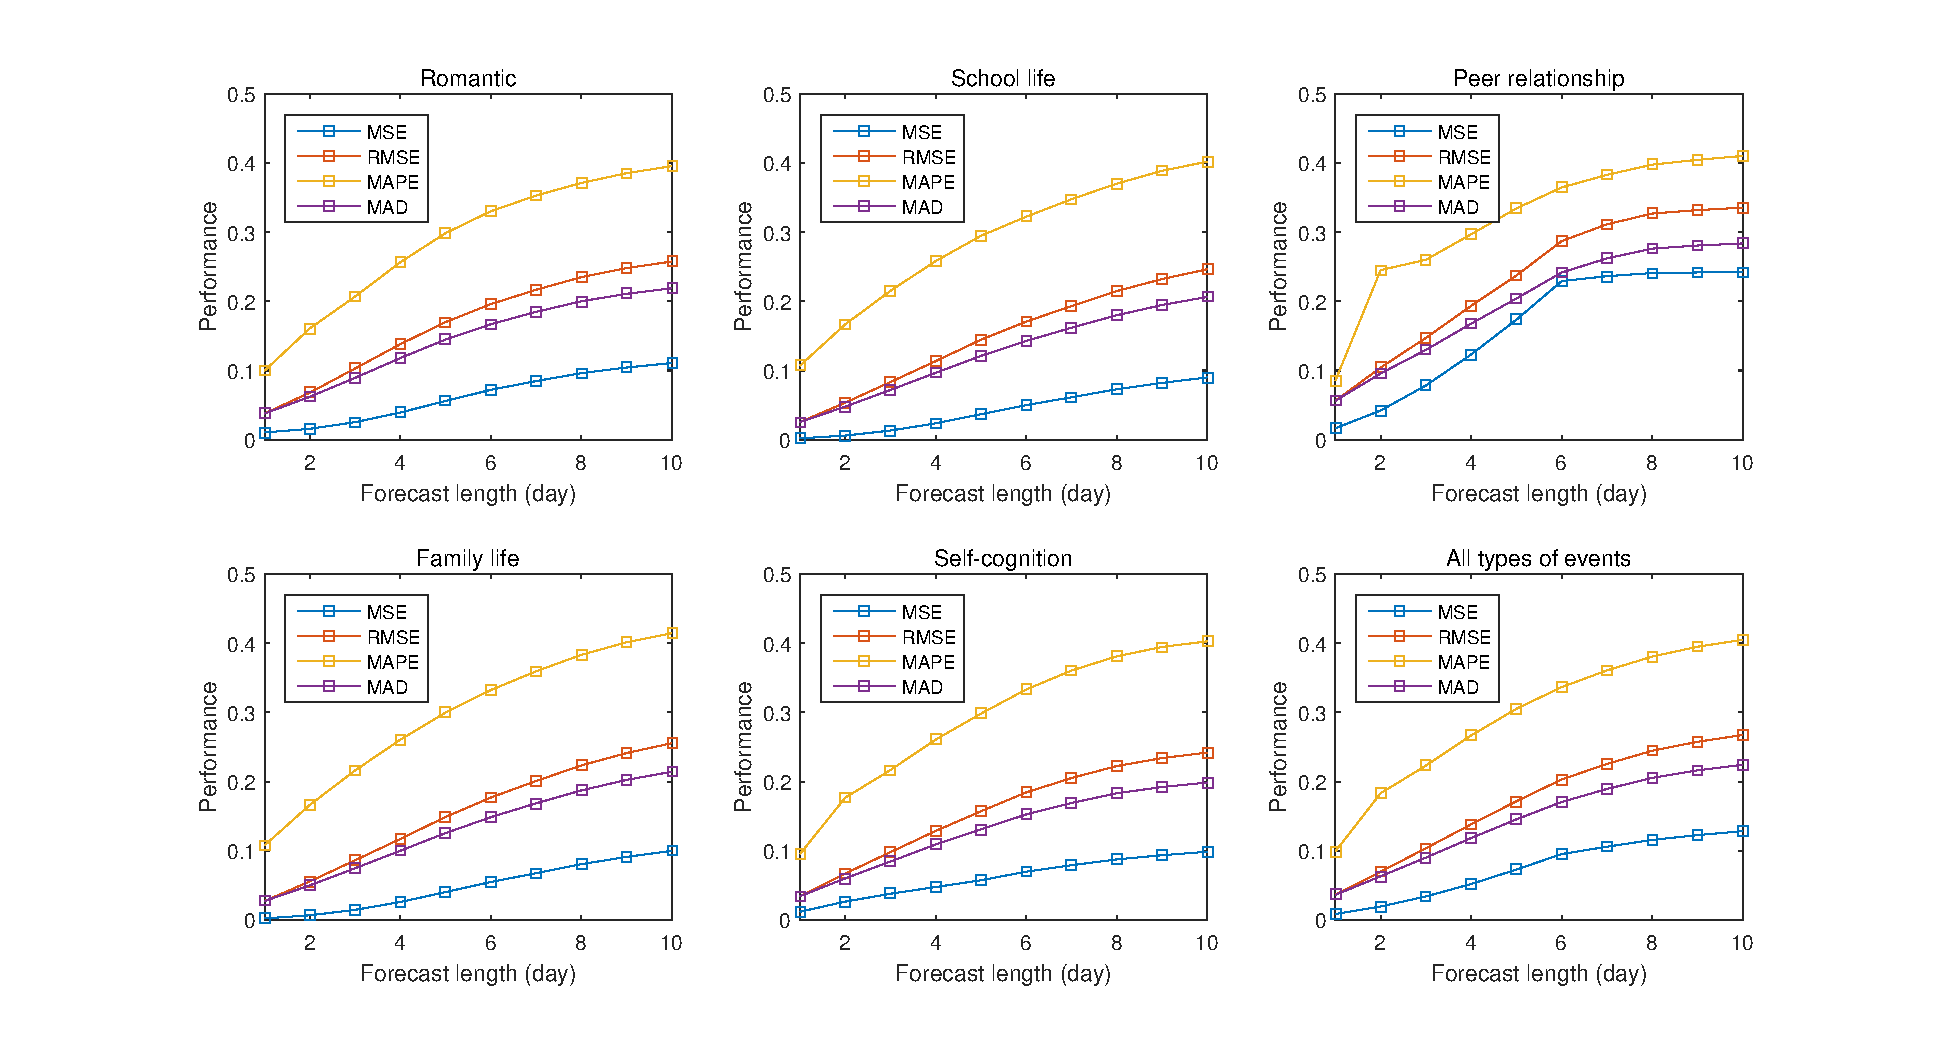
\includegraphics[width=\linewidth]{figs/predictWindow2.eps}
\label{fig:length}
\end{figure*}

\paragraph{Stress prediction performance under different observation windows}
We further explored to combine stress-buffering effects into future stress prediction under different length of observation windows, ranging from 1 to 10 days, as shown in Figure \ref{fig:length}.
With window length increasing,
prediction errors showed increasing trend in all metrics.
The reason might be that longer prediction window took more previous predicted results,
and errors accumulates with more predicted values taken into the next step prediction.
Among five dimensions of stressor events,
prediction for school life stress achieved the best performance.
One reason might be more positive events and stressors about school life events were detected from adolescents' microblogs,
providing sufficient data in prediction process.
On the other side,
stress coming from school life was the most common stress in student group,
with relative stable periodicity,
which was more suitable for current prediction model.


\begin{figure}
\centering
\caption{Stress prediction performance under L\&S\&P stress-buffering pattern of positive events.}
\includegraphics[width=\linewidth]{figs/thresh.eps}
\label{fig:thresh}
\end{figure}

\paragraph{Parameter settings}
Parameter $\alpha$ was adjusted when integrated impact of positive events into stress prediction.
For each of the four groups of stress-buffering patterns,
we adjust $\alpha$ in the effect of $\alpha \times L$.
We calculated the corresponding prediction result for each adolescent respectively,
and showed the result of whole testing group in average performance.
Figure \ref{fig:thresh} showed the changing trend under the L\&S\&P pattern.
Prediction errors decreased first and then increased,
and the best performance was achieved when $\alpha$ was nearby 0.52,
with 0.0649 MSE, 0.2548 RMSE, 0.2638 MAPE and 0.0858 MAD as the average performance of the whole experimental data set.
Multiple methods for integrating stress-buffering impact of positive event into stress prediction could be adopted in the future.
In this paper we adopted the simple one to verify the effectiveness of our model in quantifying the impact of positive events.
The setting of parameter $\alpha$ could be changed due to different individuals and data sets.
